\bibliographystyle{unsrtr}
\chapter{Translocation avec membrane fixe}
\label{translocmurfixe}

\minitoc

\newpage








\section{Préparation à la translocation}

\subsection{Définition de la membrane}

Bien que d'autres cristaux bidimensionnels existent, le graphène reste le candidat principal pour le séquençage en utilisant des nanopores dans des membranes fines. Nous avons donc considéré un modèle de membrane proche de ce dernier.
Afin de modéliser la membrane à travers laquelle notre polymère va effectuer une translocation, nous avons choisi de respecter les dimensions relatives  entre le graphène et l'ADN. Un réseau hexagonal de paramètre de maille $\frac{\sigma}{2}$ a été généré (voir figure \ref{reseau}). Le plan de graphène est suffisamment étendu pour qu'avec des conditions aux limites périodiques (pour simuler un plan infini), le polymère le plus grand utilisé ne puisse jamais se retoucher lui même, soit 5488 grains. Cette étendue importante implique que les atomes de notre membrane seront les atomes majoritaires.

\begin{figure}[H]
\begin{center}
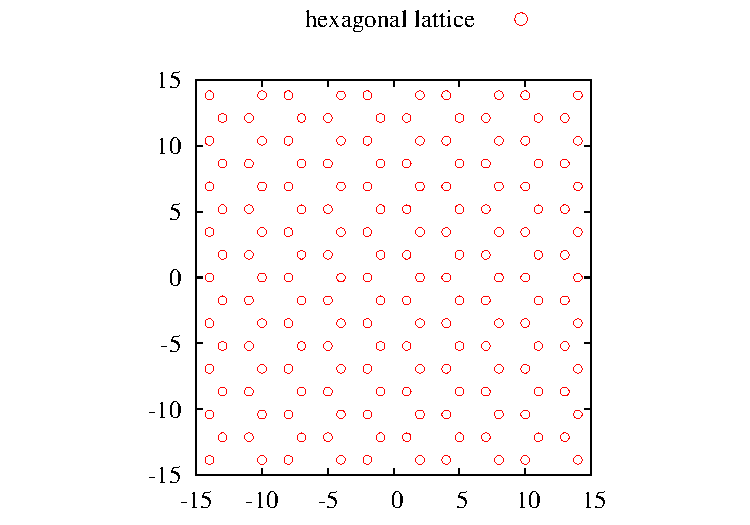
\includegraphics[width=0.65\textwidth]{lattice.pdf} 

\caption{Réseau héxagonal constituant la membrane}
\label{reseau}
\end{center}
\end{figure}

Le réseau est ensuite amputé en son centre de tous les grains situés dans un rayon fixé pour créer le pore. Dans ce chapitre, les grains de la membrane sont fixes, les équations du mouvement ne sont pas intégrées pour la membrane, elle n'existe qu'à travers l'intéraction avec le polymère par des potentiels stériques de type Lennard-Jones. Afin d'éviter que le polymère ne pénétre entre les grains de notre membrane, nous avons choisi $\sigma_{ij}=\sigma$ pour toute intéraction avec un grain de la chaîne du polymère et $\sigma_{ij}=1.25\sigma$ pour un grain latéral. Cette valeur est supérieur à l'espacement entre grains de la membrane. Physiquement, dans le cas du graphène ces tailles correspondent à la taille des orbitales atomiques de type $\pi$ du graphène avec lesquelles le polymère intéragit.


\subsection{Polymère greffé et configurations initiales}

Dans un premier temps, rappelons comme nous l'avons dans le premier chapitre que la translocation peut se dérouler dans différents contextes. Elle peut être due uniquement aux fluctuations thermiques, on parle alors de translocation non biaisée, ou être pilotée par une force extérieure, on parle alors de translocation forcée (driven translocation). Les forces extérieures peuvent être de natures variées, on citera notamment l'utilisation de champs électriques (électrophorèse), de gradients de potentiels chimiques, de flux imposé sur le solvant, ou encore l'emploi de pinces ( optiques ou magnétiques) \cite{keyser}. Nous avons choisis de nous placer dans ce dernier cas, notre polymère est donc tracté par une de ses extrémitées. En effet, l'alternative plus courante d'appliquer une force au centre du pore (ce qui représente un gradient de potentiel chimique ou électrique) impose de définir une zone d'application de la force qui est clairement définie dans les modèles simples, mais qui deviendrait vite compliquée dans les cas de déformation de la membrane, comme nous l'envisagerons au chapitre 5. Puisque nous souhaitons que les conditions soient comparables, nous obterons pour la traction de notre polymère.



Nous avons dans le premier chapitre parlé d'une barrière d'énergie à franchir pour effectuer la translocation d'un polymère, calculons la. Pour cela, nous devons dans un premier temps déterminer la probabilité de distribution d'un polymère idéal greffé à une paroi. La chaîne idéale présente comme conditions aux limites, la non pénétration des monomères à travers la paroi. On note $P(\textbf{r},\textbf{r}_0,n)$ la probabilité de trouver le $n$-ième monomère en position $\textbf{r}$, pour $n \gg 1$, le premier monomère étant greffé en $\textbf{r}_0$. $P_0$ est la distribution calculée dans le chapitre précédent pour un polymère idéal libre:

\begin{eqnarray}
P_0(\textbf{r},\textbf{r}_0,n)=\left(\frac{3}{2\pi n b^2}\right)^\frac{3}{2}\exp\left(-\frac{3(\textbf{r}-\textbf{r}_0)^2}{2 n b^2}\right)
\end{eqnarray}

A l'instar de nombreux problèmes d'électromagnétisme ou de mécanique des fluides, on utilise la méthode des images miroirs afin de déterminer $P(\textbf{r},\textbf{r}_0,n)$. En effet, on a:

\begin{eqnarray}
P(\textbf{r},\textbf{r}_0,n) \propto P_0(\textbf{r},\textbf{r}_0,n)-P_0(\textbf{r},-\textbf{r}_0,n)
\end{eqnarray}

La membrane joue alors le rôle de miroir plan (analogie optique \cite{lipson2011optical}), de conducteur (analogie électrostatique \cite{jackson1999classical}) ou encore d'obstacle sur lequel rebondi un jet (source miroir en mécanique des fluides \cite{kundu2008fluid}).

Dans le cas idéal, la probabilité de distribution du monomère de queue est à variables séparables. En posant $\textbf{r}_0= \epsilon y$ avec $\epsilon \ll 1$, un développement limité au premier ordre donne:

\begin{eqnarray}
P(\textbf{r},\textbf{r}_0,n) \propto \left(\frac{3}{2\pi n b^2}\right)^\frac{3}{2} \left(\frac{6 y \epsilon}{n b^2}\right)\exp\left(-\frac{3\textbf{r}^2}{2 n b^2}\right)
\end{eqnarray}

Cette probabilité est à variables séparables, c'est à dire qu'elle peut s'écrire comme le produit d'une fonction de x, d'une fonction de y  et d'une fonction de z. Selon x et z (la membrane occupant le plan y=0), la distribution reste inchangée (et donc gaussienne) par rapport au cas du polymère libre, il n'y a une influence sur les configurations interdites par la membranes que selon l'axe y.

Pour le cas d'un polymère non idéal, les termes supplémentaires introduits dans $P_0$ ne permettent pas de séparer les variables et d'obtenir une expression analytique. Cependant l'allure de la distribution du monomère de queue reste proche du cas idéal tout en présentant des caractéristiques dues au volumes exclus (voir figure \ref{polagainstwall}). Afin d'aborder la translocation, nous avons du créer des configurations indépendantes de polymères à l'équilibre, juste avant l'application d'une force. Lors de ce processus de génération, nous avons laissé le polymère évoluer librement en fixant une extrémité au centre du pore. Les 1000 configurations initiales sont toutes séparées d'au moins dix temps de corrélation du polymère.


\begin{figure}[H]
\begin{center}


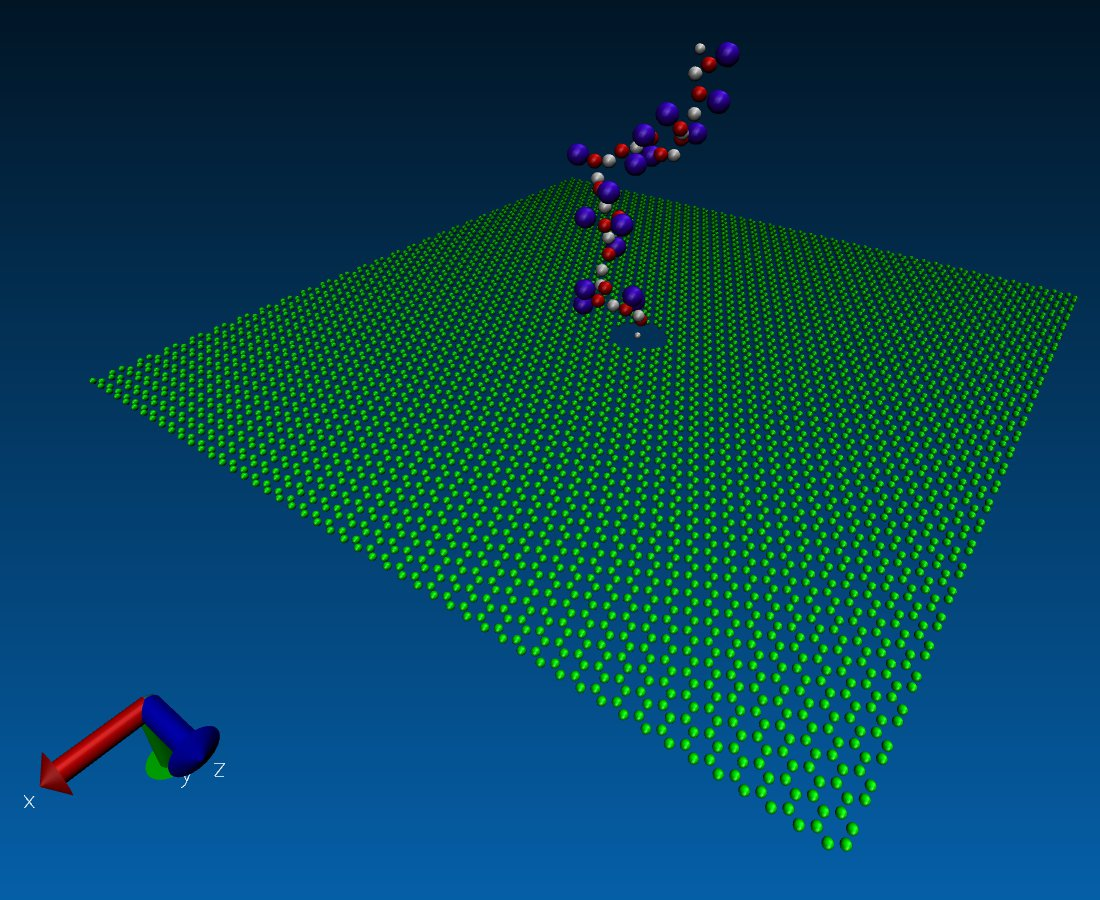
\includegraphics[width=0.7\textwidth]{confinit.jpg}
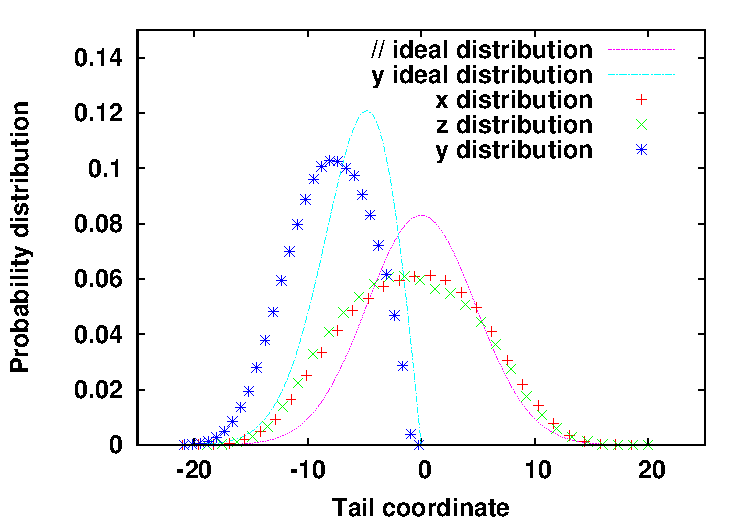
\includegraphics[width=0.9\textwidth]{probdistribution.pdf}


\caption[Polymère greffé sur une membrane]{En haut: Capture d'écran d'une configuration de notre polymère structuré évoluant avec une extrémitée fixée au centre du nano-pore. En bas, probabilité de distribution théorique du monomère de queue pour un polymère idéal et résultats numériques pour un polymère à monomères durs (N=16 grains latéraux). Parallèlement à la membrane, la distribution gaussienne idéale est aplatie au centre à cause de la zone d'exclusion des autres monomères. De même pour la direction perpendiculaire, le pic maximum est repoussé par la présence d'autres monomères. Dans les deux cas, l'éloignement maximal n'est pas modifié car le cas idéal correspond déjà à des chaînes étirées sans superpositions de monomères. }
\label{polagainstwall}
\end{center}
\end{figure}


\subsection{Théories de la translocation non biaisée}


La probabilité de distribution du polymère accolé à une membrane permet, à partir de la fonction de partition stérique, $Z_S(n)= \int_{y>0} P(\textbf{r},\textbf{r}_0,n) \textbf{dr}$, de calculer l'énergie libre d'origine entropique d'un tel système. Dans la limite $n \gg 1$, le premier terme non nul du développement limité impose la loi d'échelle: $Z_S(n) \propto n^{\gamma'-1}$ (on aura un facteur $\gamma'$=1/2 pour un polymère gaussien, 0.68 pour un polymère avec volumes exclus,  ($\nu$=0.588) ou 1 pour une chaine rigide). Pour un polymère de $N$ monomères en cours de translocation, lors du passage du $n$-ième monomère, Sung et Park \cite{Sung1996} décrirent les premiers la valeur de l'énergie libre en prenant en compte les effets entropiques de part et d'autre de la membrane:
\begin{eqnarray}
F(N,n)= -k_BT\ln\left(Z_S(n)Z_S(N-n)\right)= \frac{1}{2} k_BT \ln \left(n(N-n)\right) +cste
\label{energbar}
\end{eqnarray}

Cette barrière d'énergie à franchir au cours de la translocation peut être altérée en appliquant une différence de potentiel, chimique ou électrique, ou encore en appliquant directement une force sur la chaîne. La Figure \ref{energiebarrier} montre cette barrière d'énergie.
 Dans le cas d'un polymère non idéal avec volumes exclus, Muthukumar \cite{Muthukumar1999} a montré que l'équation du polymère idéal \ref{energbar} était une simplification de l'équation suivante plus générale:

\begin{eqnarray}
\frac{F(N,n)}{k_BT}= (1-\gamma_2')\ln(n)+ (1-\gamma_1')\ln(N-n)+cste
\label{energbarsaw}
\end{eqnarray}

avec $\gamma_i'$ l'exposant caractéristique de la taille du polymère dans le milieu i ($\gamma_i'$=0.5 pour un polymère idéal ou un milieu saturé en polymère,$\gamma_i'$=0.68  pour un polymère avec volumes exclus ($\nu$=0.588) ou encore 1 pour des polymères ultra rigides ou rod-like en anglais).

Dans le cas général, $\gamma_1'$=$\gamma_2'$ et la translocation est biaisée par une différence de potentiel (chimique, électrique...), on alors la relation:

\begin{eqnarray}
F(N,n)= -k_BT(1-\gamma')\ln \left(n(N-n)\right) + n \Delta \mu +cste
\label{energbargen}
\end{eqnarray}

Dans notre cas, nous n'avons pas une différence d'énergie qui s'applique à la barrière entropique, mais la contribution du travail d'une force (sa transmission le long de la chaîne sera discutée avec les résultats).

Sung, Park et Muthukumar \cite{Sung1996,Muthukumar1999} utilisent cette énergie pour résoudre l'équation dite de Fokker-Planck qui traite l'évolution de la probabilité d'avoir $n$ monomères qui ont effectué la translocation:
\begin{eqnarray}
\frac{\partial P(n,t)}{\partial t} =   \mathcal{L}_{FP}(n) P(n,t)
\label{equfokkerplank1}
\end{eqnarray}

Avec l'opérateur $\mathcal{L}_{FP}(n)= (1/b^2)(\partial/\partial n) D(n)[exp(-F(N,n)/k_BT)](\partial/\partial n)[exp(F(N,n)/k_BT)]$

Chuang Kantor et Kardar \cite{Chuang2001} notèrent que cette équation, dans le cas non biaisé, peut être réduite à:

\begin{eqnarray}
\frac{\partial P(n,t)}{\partial t} =   \frac{\partial ^2 P(n,t)}{\partial ^2 n} +(1-\gamma') \frac{\partial  }{\partial  n}\left(P(n,t)\frac{1-2n}{(1-n)n}\right)
\label{equfokkerplank2}
\end{eqnarray}
grace aux changements de variable:
$n \rightarrow nN$ et $t \rightarrow tD/N^2$


Gardons à l'esprit que ces équations sont valables dans la mesure où le polymère demeure à l'équilibre thermodynamique au cours de la translocation.



\begin{figure}[H]
\begin{center}
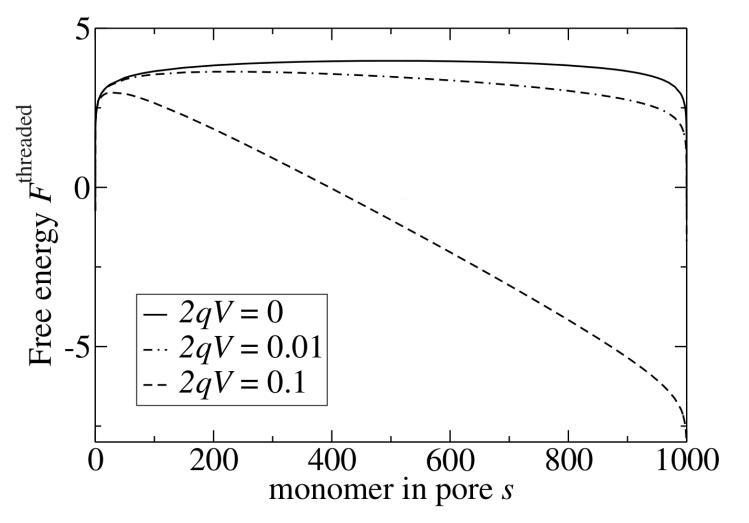
\includegraphics[width=0.7\textwidth]{transelec.jpg} 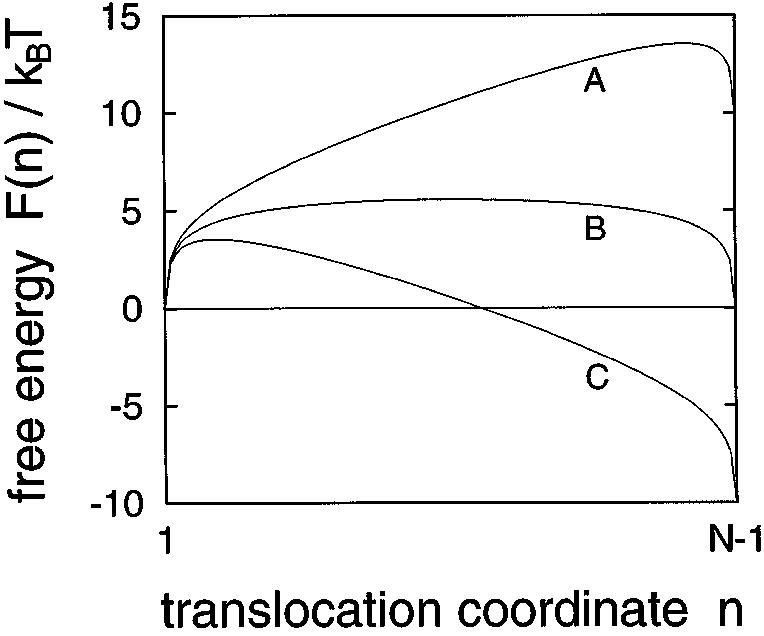
\includegraphics[width=0.5\textwidth]{transpotchim.jpg}

\caption[Translocation, barrière d'énergie d'origine entropique]{Modification de la barrière entropique par une différence de potentiel électrique (en haut \cite{these}) et de potentiel chimique (en bas \cite{Sung1996}). A: différence de potentiel opposée à la translocation, B: différence de potentiel nulle, C: différence de potentiel favorable.}
\label{energiebarrier}
\end{center}
\end{figure}

L'équation précédente \ref{equfokkerplank2} ne faisant plus apparaître $N$, on peut en déduire qu'il existe un paramètre $\alpha$ universel qui permet de décire le temps de translocation.
\begin{eqnarray}
\tau \propto N^\alpha
\label{tauunbiased}
\end{eqnarray}


 Reste à déterminer $\alpha$. En utilisant des conditions aux limites appropriées (réfléchissante en 0 pour empêcher le retour du polymère et absorbante en bout de chaîne) la résolution de l'équation de Fokker-Planck donne $\tau \propto N^{2}/D$. Le coefficient de diffusion a utiliser est sujet de discorde, Sung et Park \cite{Sung1996} considèrent le coefficient de diffusion comme étant celui du polymère libre et donc inversement proportionnel à $N$ (voir chapitre 2), ce qui leur fait prédire $\tau \propto N^{3}$, Muthukumar \cite{Muthukumar1999} lui, considére que c'est le coefficient de diffusion du polymère au sein du pore qui est pertinent (D est donc une constante) d'où son affirmation $\tau \propto N^{2}$. Cependant, ses exposants sont vite remis en question par Chuang, Kantor et Kardar \cite{Chuang2001}. Ils arguent que le temps de translocation ne peut pas être plus court que le temps de relaxation du polymère, proportionnel à $N^{1+2\nu}$(comme nous l'avons vu au chapitre 2), qui est caractéristique d'un déplacement du polymère sur une distance de l'ordre de son rayon de giration (comme si il n'y avait pas de membrane à franchir). Si l'exposant associé au temps de translocation est plus faible que le temps de relaxation, cela voudrait dire que la chaîne n'a pas le temps de s'équilibrer au cours de la translocation et donc qu'on ne peut pas appliquer l'équation de Fokker-Planck au système. On alors un phénomène de translocation sous-diffusif. Des essais de résolution ont été menés en utilisant une équation de Fokker-Planck fractionnelle \cite{Metzler2003} (qui s'applique dans un cas plus général) et trouvent $\tau \propto N^{2+2\nu-\gamma'}$. Une approche suggère une translocation avec plusieurs échelles de temps représentant l 'équilibration des liaisons et la diffusion, on aurait alors $\tau \propto N^{2+\nu}$. La dernière tentative d'approche théorique en date est à partir de l'équation de Langevin généralisée \cite{Panja2010} et prédit $\tau \propto N^2$ pour un polymère idéal, $\tau \propto N^{2+\nu}$ dans le cas de Rouse et $\tau \propto N^{1+2\nu}$ dans le cas de Zimm (avec intéractions hydrodynamiques). Les simulations numériques effectuées n'apportent pas de consensus et estiment des exposants compris entre 2.2 et 2.6, suggérant une forte dépendance aux conditions de simulation et une possibilité d'existence de différent régimes en fonction de l'importance de la friction. En effet une transition entre les deux exposants $1+2\nu$ et $2+\nu$ a été reportée \cite{Panja22010}.\\

\subsection{Théories de la translocation forcée}

La question de la translocation non biaisée qui ne fait pas consensus n'a pas empécher la communauté scientifique d'aborder le cas de l'introduction d'une force pour faciliter le phénomène. Il vient naturellement à l'esprit que la contribution d'une force appliquée vers le côté trans va favoriser la translocation et on s'attend donc à pouvoir décrire le temps de translocation de la manière suivante, toujours avec un paramètre $\alpha$ caractéristique du nombre de monomère et un nouvel exposant critique $\delta$ pour la force:

\begin{eqnarray}
\tau \propto N^\alpha / f^\delta
\label{taubiased}
\end{eqnarray}

il est évident que l'amplitude de la force va influer sur la valeur des exposants critiques $\alpha$ et $\delta$. dans le cas d'une force extrémement faible, on s'attend à se retrouver dans le cas précédent de la translocation non biaisée avec $\alpha$ compris entre 2.2 et 2.6. En ce qui concerne l'autre extrème, une force très importante, la translocation est entièrement régie par la force (il n'y a plus la moindre influence de la température) et on attend $\tau \propto N/f$.
 La pluspart des études théoriques et numériques se concentrent sur le cas de l'application de la force au sein du pore. Le cas du polymère tracté est plus rarement abordé.
 Dans le cas général, l'hypothèse de quasi-équilibre utilisée pour résoudre analytiquement le cas de la translocation non biaisée est maintenant encore moins pertinente avec l'ajout d'une force. Il est possible de définir une limite inférieure à la valeur de $\alpha$. En effet si on considère le cas de l'application d'une force en l'absence de membrane, la translocation est effectuée quand le polymère a franchi une membrane virtuelle, il a donc été déplacé sur une distance de l'ordre de son rayon de giration. Or avec la friction, la vitesse moyenne du centre de masse s'écrit: $v \propto f/N$, d'où $\tau \propto N^{1+\nu}/f$. On a donc $\alpha=1+\nu$ comme limite inférieure.
 
 
 

 \cite{Kantor2004} traction
 
 \cite{Ikonen2012} tail retractation intopore
  \cite{ Huopaniemi2007} tail retractation pulling

 
 \textcolor{red}{revoir les 3 régimes proposés par sakaue}
 ces théories n ont pas été testées sur un polymère tracté pour la transloc
 
 
 \begin{figure}[H]
\begin{center}
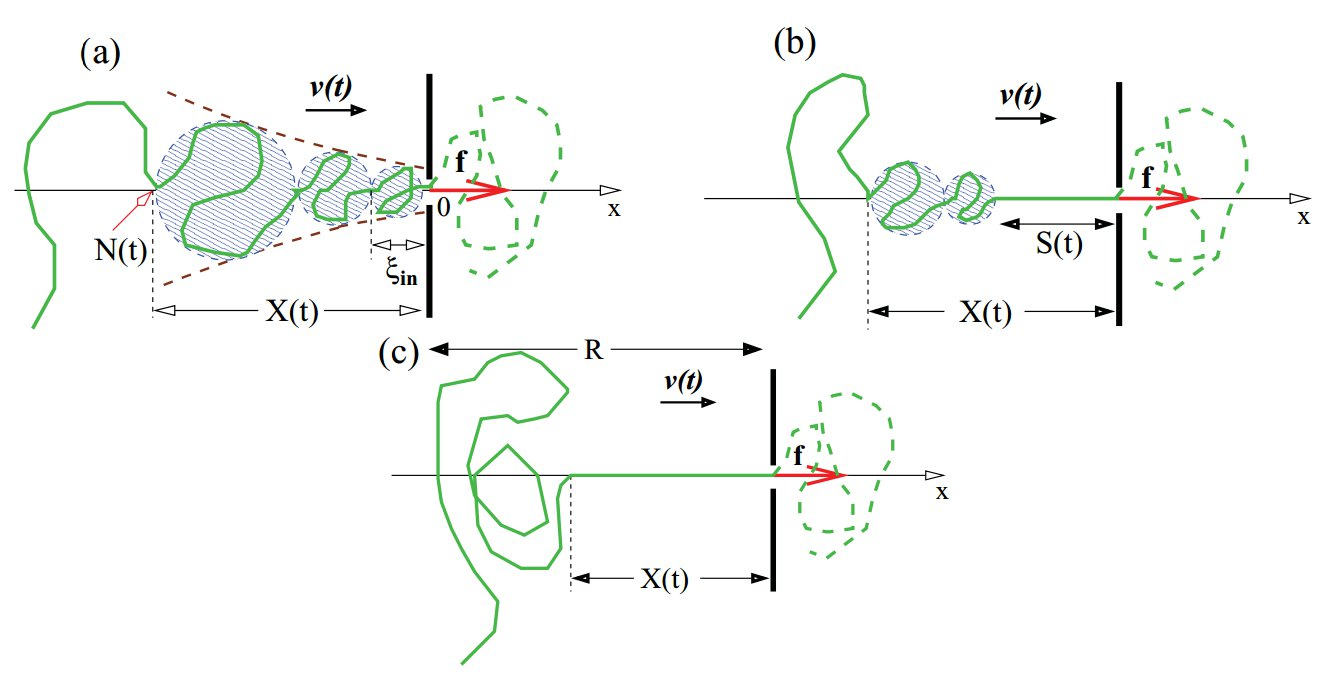
\includegraphics[width=0.95\textwidth]{regimeprofiles.jpg}
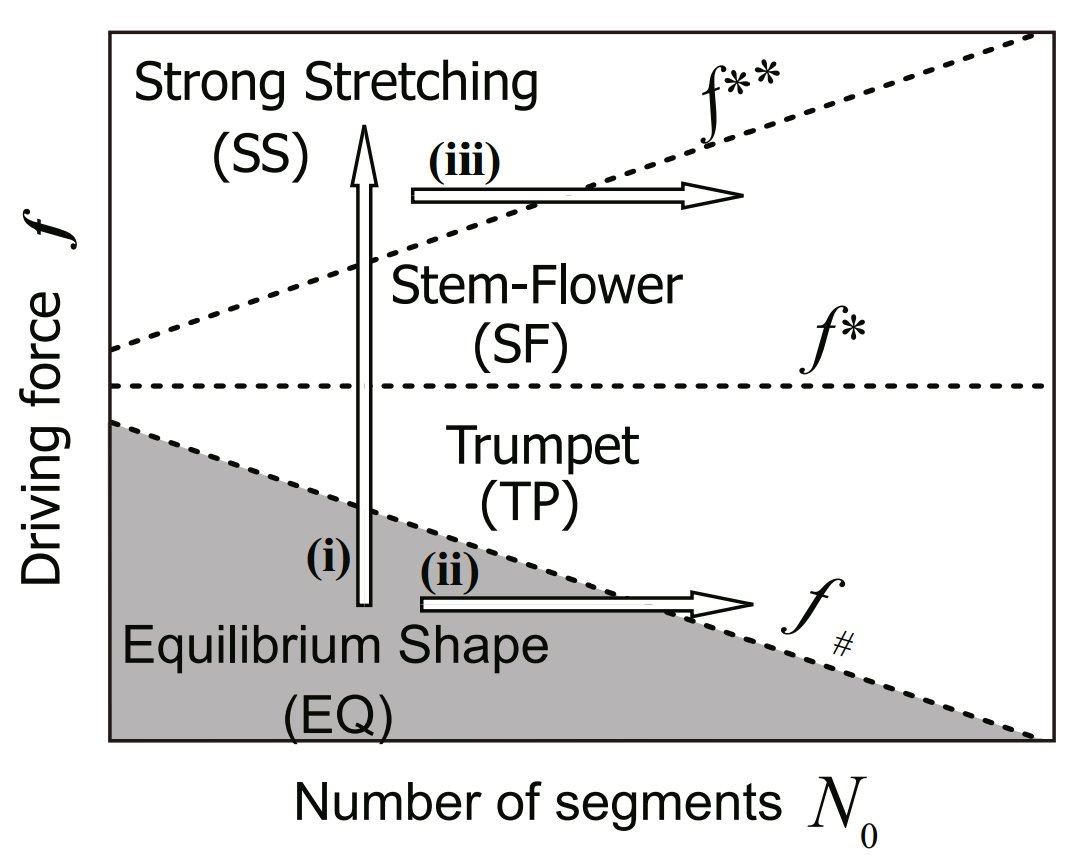
\includegraphics[width=0.5\textwidth]{regimedistrib.jpg} 

\caption[Régimes possibles au cours de la translocation]{Régimes proposés par Sakaue.}
\label{regimeprofiles}
\end{center}
\end{figure}

 \begin{figure}[H]
\begin{center}
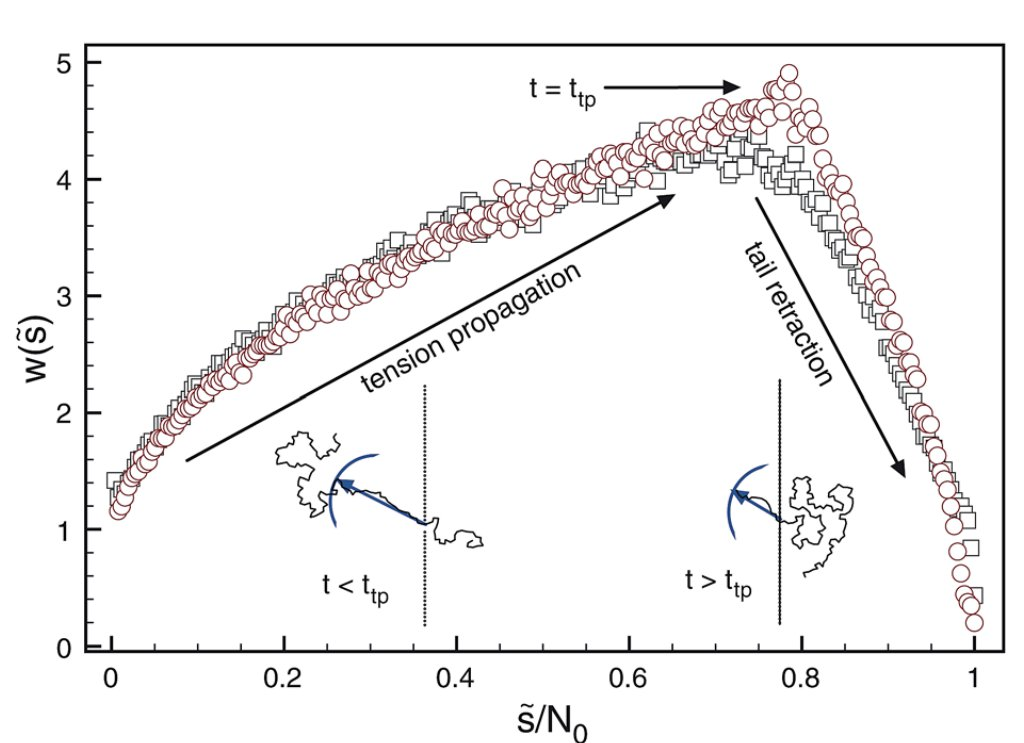
\includegraphics[width=0.75\textwidth]{tailretractinpore.jpg}
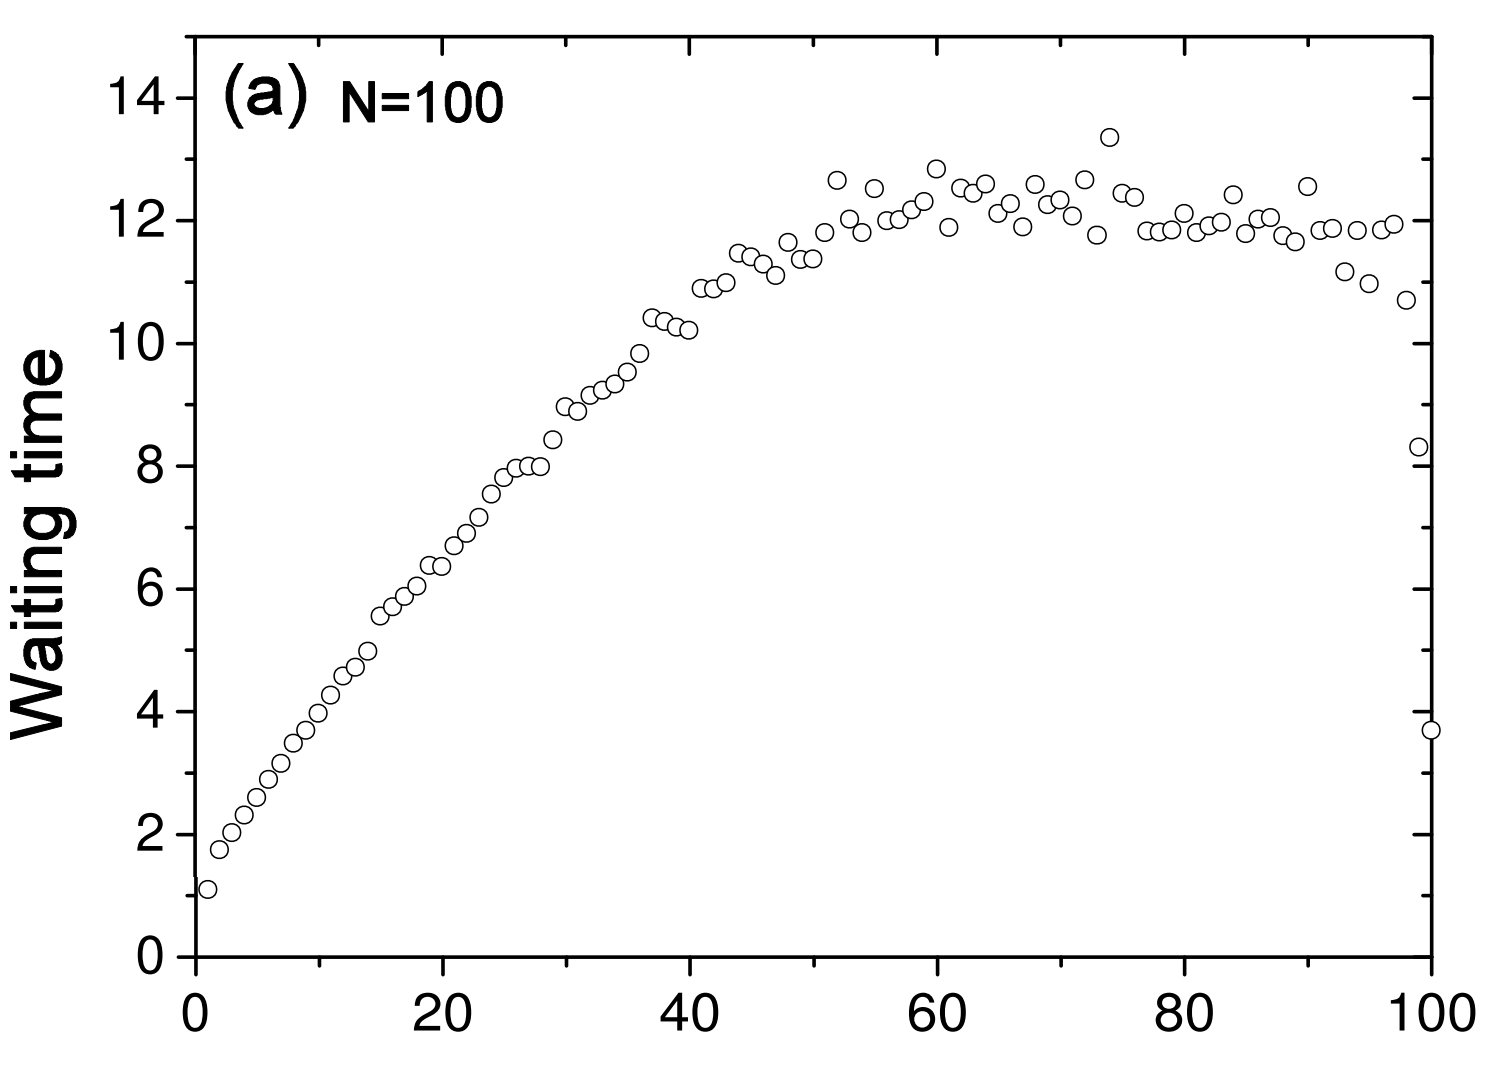
\includegraphics[width=0.75\textwidth]{tailretractpulling.jpg} 

\caption[Temps d'attente et rétractation de la queue du polymère]{Rétractation de la queue.}
\label{regimeprofiles}
\end{center}
\end{figure}

 
 Nous avons étudié trois cas différends dans le cadre de notre travail sur une membrane fixe. Dans un premier temps, la translocation d'un polymère non structuré à travers un pore suffisamment large pour limiter les frottements est expérimentée. Nous avons retiré 24 grains du centre de la membrane pour former le nanopore. Puis nous avons testé notre polymère structuré, également dans un pore suffisamment large, il a alors fallut retirer 54 grains. Pour terminer nous avons investigué l'effet d'un nanopore étroit sur la translocation du polymère structuré en retournant à un pore constitué par le retrait de 24 grains. les deux pores utilisés sont présentés sur la figure \ref{bothpores}.
 \begin{figure}[H]
\begin{center}
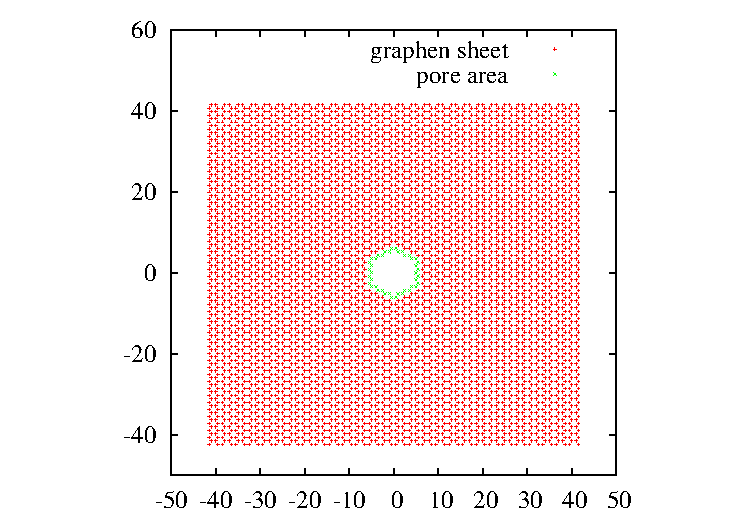
\includegraphics[width=0.45\textwidth]{holebigger.pdf} 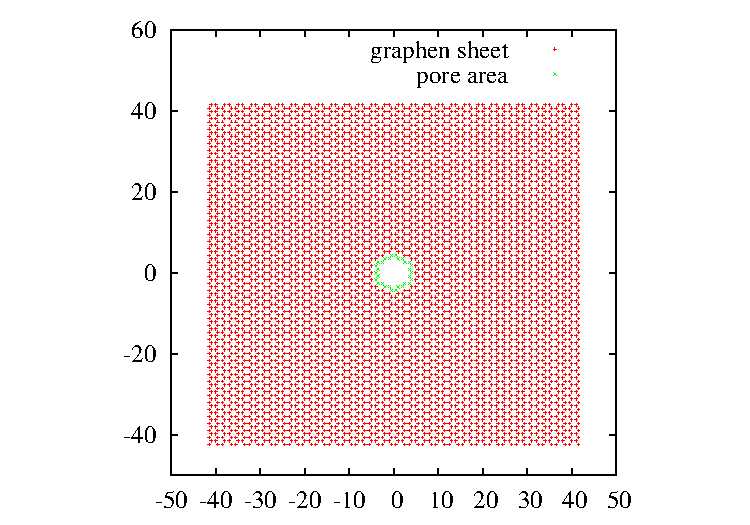
\includegraphics[width=0.45\textwidth]{holesmall.pdf}

\caption[Nanopores utilisés]{Les deux nanopores nanopores utilisés. A gauche: Pore large pour la translocation de polymères structurés. A droite: Pore étroit pour la translocation de polymères structurés et larges pour des polymères simples linéaires. Un zoom sur les pores et la taille relative des grains du polymère en cours de translocation seront fournis par la suite  pour chaque expérience.}
\label{bothpores}
\end{center}
\end{figure}

\subsection{Distribution du temps de translocation}

Dans leurs travaux sur la translocation, Daniel Y Ling et Xinsheng Sean Ling \cite{Ling2013} proposent d'étudier la distribution des temps de translocation en considérant la translocation comme un phénomène de diffusion biaisée unidimensionelle. Ils considérent le pore suffisamment fin comparé à la longueur du polymère pour être considéré comme un marcheur qui se déplace le long de ce dernier. Ils peuvent donc lui appliquer l'équation de Fokker-Planck:

\begin{eqnarray}
\frac{\partial P(x,t)}{\partial t} =   D\frac{\partial ^2 P(x,t)}{\partial ^2 x} - \nu \frac{\partial  P(x,t)}{\partial  x}
\label{equfokkerplank}
\end{eqnarray}

Avec $P(x,t)$ la probabilité pour le pore d'être à la coordonnée $x$ le long du polymère à l'instant $t$, $D$ le coefficient de diffusion et $\nu$ la vitesse du marcheur. Ils utilisent pour conditions aux limites, le premier monomère au sein du pore à $t=0$ et une absorption lorsque le pore atteint $L$ l'extrémité du polymère, il n'y a pas de retour possible:

\begin{eqnarray}
 P(x,0) =   \delta(x)\text{  }, \text{  } P(L,t)=0
\label{condlim}
\end{eqnarray}

La solution de l'équation différentielle est:

\begin{eqnarray}
 P(x,t) = \frac{1}{\sqrt{4\pi D t}} \left(e^{-\left(x-\nu t\right)^{2}/4Dt} -e^{(\nu L/D)}e^{-\left(x-2L-\nu t\right)^{2}/4Dt} \right)
\label{equfokkerplanksol}
\end{eqnarray}

La distribution du temps de translocation est la distribution du temps de premier passage:

\begin{eqnarray}
 F1(t) = -\frac{d}{dt}\int_{-\infty}^L  P(x,t) dx
\label{firstpassageint}
\end{eqnarray}

\begin{eqnarray}
 F1(t) = \frac{L}{\sqrt{4\pi D t^3}} \left(e^{-\left(L-\nu t\right)^{2}/4Dt}\right)
\label{firstpassage}
\end{eqnarray}

Avec l'équation \ref{firstpassage} ils arrivent à reproduire des résultats expérimentaux dans certaines conditions où la vitesse du marcheur peut être aisément reliée aux conditions expérimentales, les hypothèses $D$ et $\nu$ constants valables. Nous nous servirons de cette équation pour analyser les distributions de nos temps de translocation.


\section{Translocation du polymère simple}

\begin{figure}[H]
\begin{center}
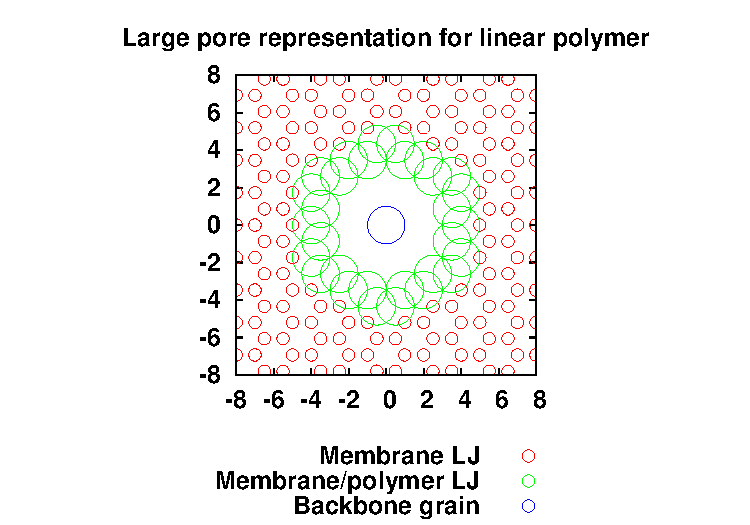
\includegraphics[width=0.9\textwidth]{simplepolpore.pdf}


\caption[Polymère simple dans le pore]{Pore large utilisé pour la translocation de notre polymère structuré. Les tailles des différents grains sont respectées. }
\label{porelargesimplepol}
\end{center}
\end{figure}




 
 
\begin{figure}[H]
\begin{center}
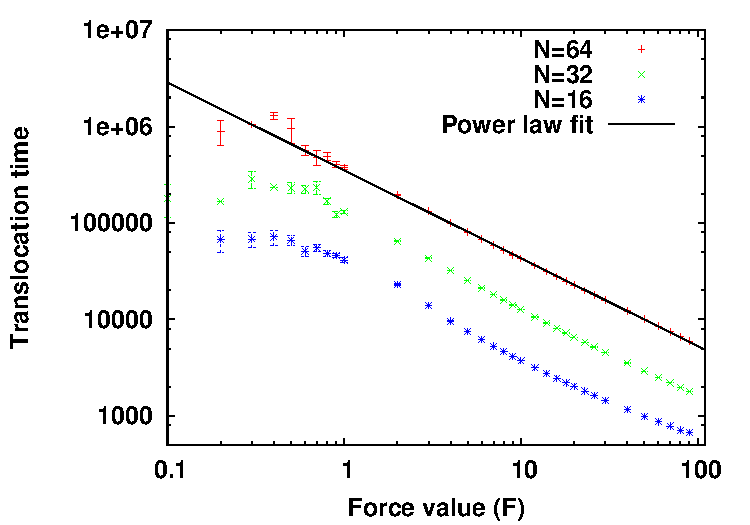
\includegraphics[width=0.85\textwidth]{translocpolsimple.pdf} 
\caption[Temps de translocation du polymère simple]{Temps de translocation moyen du polymère en fonction de la force de traction exercée.}
\label{taupolsimple}
\end{center}
\end{figure}

\begin{figure}[H]
\begin{center}
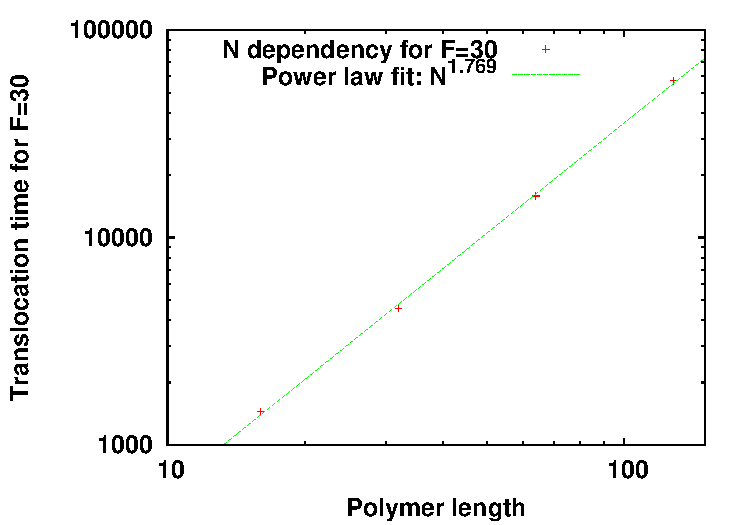
\includegraphics[width=0.85\textwidth]{ndeppolsimple.pdf}


\caption[Temps de translocation en fonction de N]{Evolution du temps de translocation moyen avec N. }
\label{ndeppolsimple}
\end{center}
\end{figure}

\begin{figure}[H]
\begin{center}
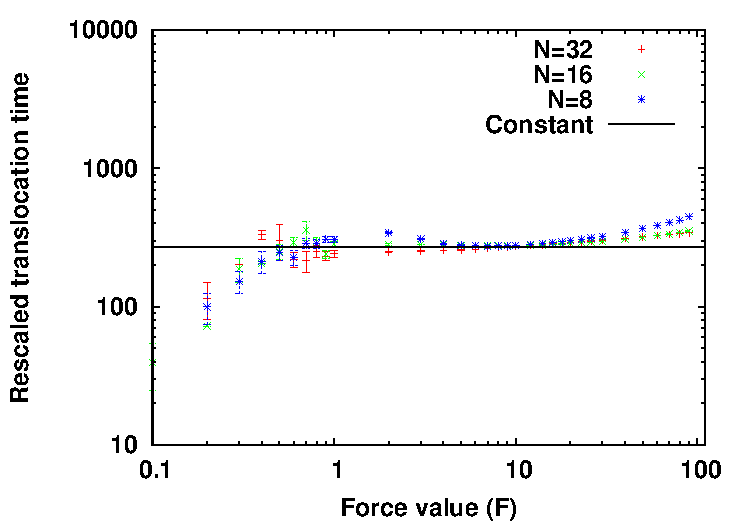
\includegraphics[width=0.85\textwidth]{transloctaufrescsimplepol.pdf}


\caption[Temps de translocation réajusté]{Temps de translocation réajusté en fonction de la force exercée. }
\label{simplepolrescale}
\end{center}
\end{figure}

\begin{figure}[H]
\begin{center}
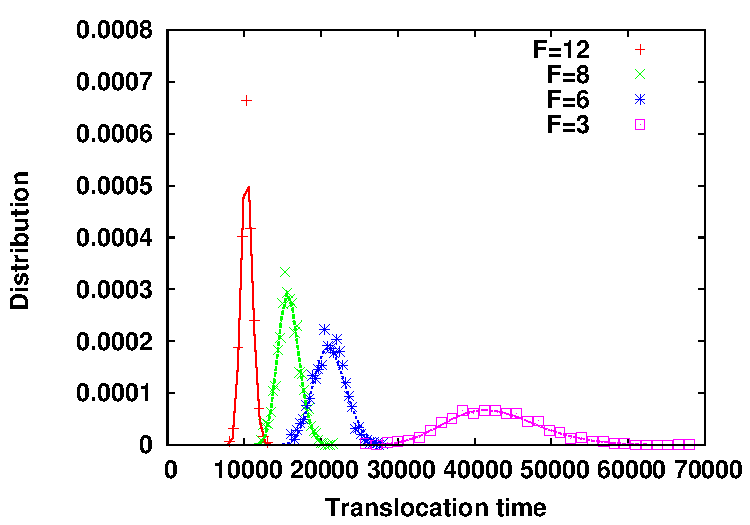
\includegraphics[width=0.85\textwidth]{distribpolsimple.pdf}


\caption[Distribution des temps de translocation du polymère simple]{Distribution des temps de translocation. }
\label{distribpolsimple}
\end{center}
\end{figure}


\begin{figure}[H]
\begin{center}
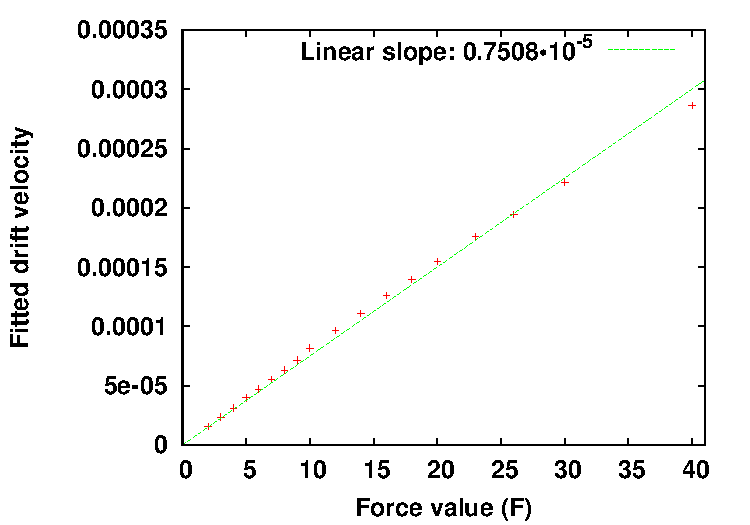
\includegraphics[width=0.85\textwidth]{translofrictioncoeffsimplepol.pdf}


\caption[Friction et translocation, polymère simple]{Estimation du coefficient de friction. }
\label{frictionpolsimple}
\end{center}
\end{figure}




 

 


\section{Translocation du polymère structuré, pore large}

\begin{figure}[H]
\begin{center}
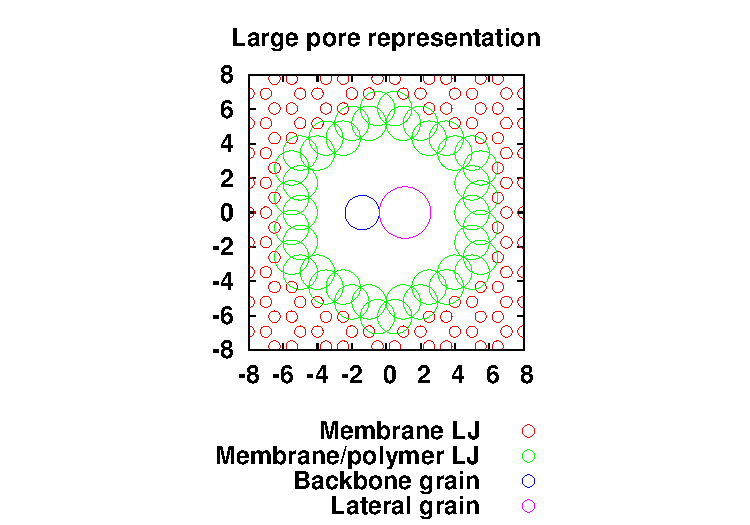
\includegraphics[width=0.9\textwidth]{largepore.pdf}


\caption[Polymère structuré et pore large]{Pore large utilisé pour la translocation de notre polymère structuré. Les tailles des différents grains sont respectées. }
\label{porelarge}
\end{center}
\end{figure}

  Le nanopore est créé en supprimant 54 grains au centre ( voir figure \ref{porelarge}). L'extrémité du polymère est alors tirée par l'ajout d'une force perpendiculaire à la membrane et d'amplitude modulée sur 3 ordres de grandeurs, de 0.1 à 100 unités de ennard-Jones (soit entre 0.067 et 67 en unité de force réduite). Un cylindre de sécurité est implanté dans le code pour vérifier que le pore est toujours peuplé. Lorsque ce n'est plus le cas, nous vérifions si le polymère a terminé sa course du coté cis ou du coté trans. En effet, pour de faibles forces, le polymère peut dans certaines simulations, ne pas effectuer la translocation.




Trois polymères ont été étudiés, ils présentent 8, 16 et 32 grains latéraux (soit une longueur de cha\^ine de 16, 32 et 64 grains respectivement). La figure \ref{holebiggertau} présente les temps de translocation moyens en fonction de la force de traction du polymère.

\begin{figure}[H]
\begin{center}
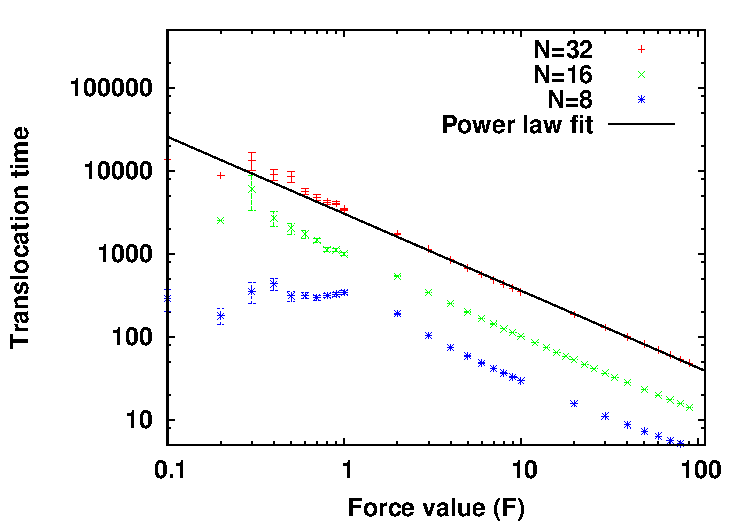
\includegraphics[width=0.9\textwidth]{translocholebigger.pdf} 
\caption[Temps de translocation du polymère structuré avec un pore large]{Temps de translocation moyen du polymère en fonction de la force de traction exercée. La rupture de pente du cas $N=8$ est imputée à des effets de taille finie, en effet le processus d'amorçage de la translocation est plus lent que la diffusion du polymère qui est elle élevée pour les chaînes courtes (variation en 1/N). On a donc moins d'événements et la diffusion semble empécher les translocations les plus longues. }
\label{holebiggertau}
\end{center}
\end{figure}



\begin{figure}[H]
\begin{center}
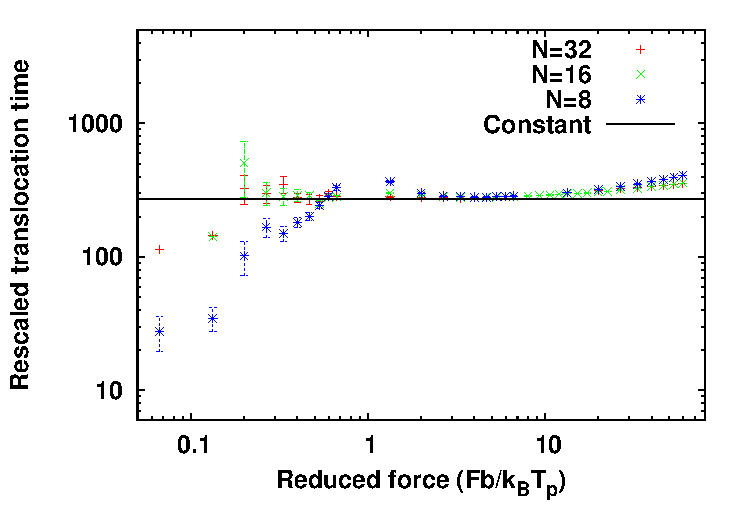
\includegraphics[width=0.9\textwidth]{transloctaufrescholebigger.pdf} 
\caption[Temps de translocation réajusté du polymère structuré avec un pore large]{sf}
\label{holebiggerescale}
\end{center}
\end{figure}

\begin{figure}[H]
\begin{center}
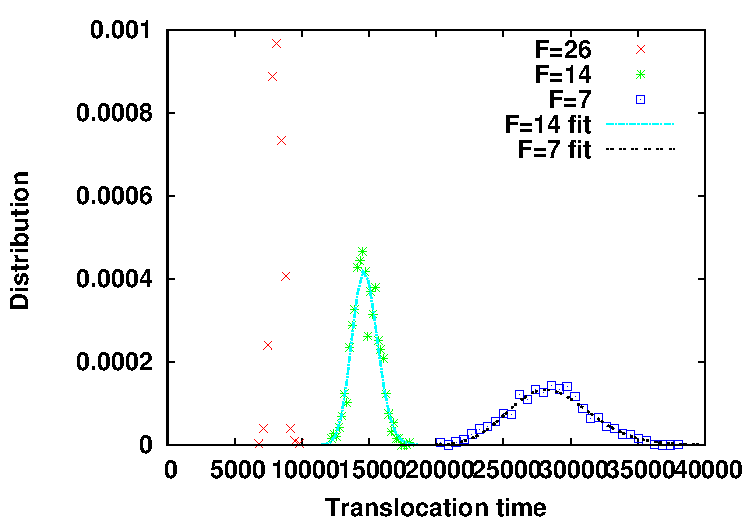
\includegraphics[width=0.9\textwidth]{distriblargepore.pdf} 
\caption[Distribution des temps de translocation du polymère structuré avec un pore large]{distrib}
\label{holebiggerdistrib}
\end{center}
\end{figure}




\begin{figure}[H]
\begin{center}
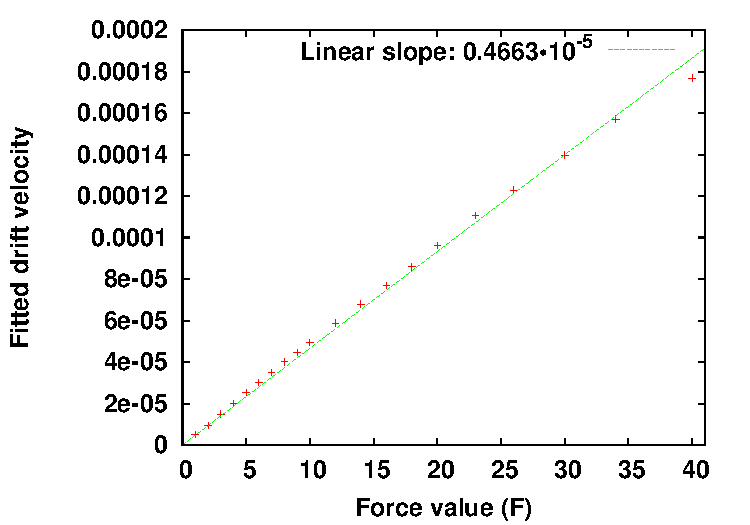
\includegraphics[width=0.9\textwidth]{translofrictioncoefflargepore.pdf}
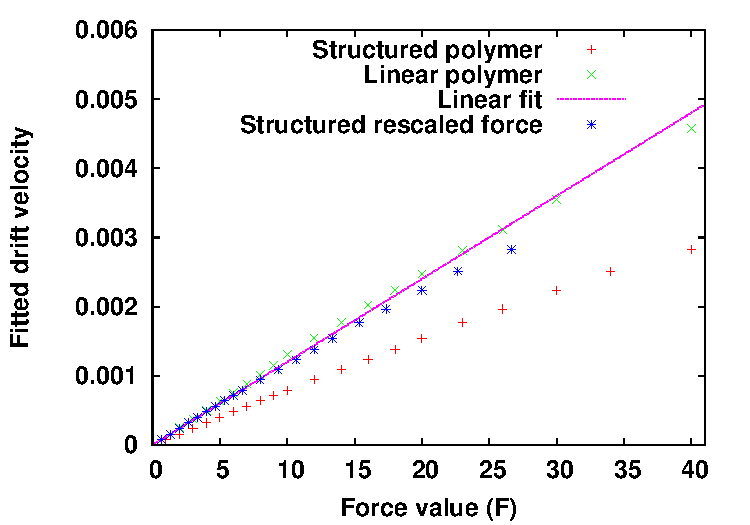
\includegraphics[width=0.9\textwidth]{largeporesfirction.pdf}



\caption[Friction et translocation, polymère structuré avec un pore large]{Estimation du coefficient de friction.}
\label{frictionholebigger}
\end{center}
\end{figure}



Exercer des forces plus faibles nous ferait perdre beaucoup trop d'événements. Afin de balayer de larges domaines, il pourrait être intéressant de travailler, comme cela peut être fait expérimentalement à vitesse de traction imposée (la force n'est alors plus constante).



Afin de ralentir la translocation, enjeu clé du séquençage, nous allons maintenant étudier l'influence d'un nanopore plus étroit. En quoi le frottement important induit par le pore va-t-il modifier les lois d'échelle trouvées précédemment?






A l'instar des prédictions de J. L. A. Dubbeldam et collaborateurs \cite{traction}, nous observons deux régimes distincts caractérisant la dépendance de la loi d'échelle avec la force. En effet, on observe à forces faibles (excepté pour $N=8$) et intermédiaires un comportement tel que $\tau \propto 1/F$. Pour des forces plus élevées, on trouve une loi d'échelle avec un exposant plus élevé ($\tau \propto F^{-0.74}$ pour N=8) Cet exposant plus élevé montre la transition vers $\tau \propto F^{(1/\nu) -2}$. La valeur plus faible qu'attendue peut être attribuée aux effets de taille finie et à l'amplitude de la force qui n'est pas assez élevée. De plus la transition entre les régime semble apparaitre plus tôt pour les $N$ faibles, contrairement à la prédiction de J. L. A. Dubbeldam et collaborateurs \cite{traction}. Cette différence pourrait venir du fait que nous tractons notre polymère (force en bout de chaîne), alors que dans leur cas, une différence de potentiel est appliquée (force au sein du pore). La Figure \ref{holebigger} permet de mieux visualiser ces régimes. En ce qui concerne l'évolution de $\tau$ avec $N$, on trouve un exposant de 1.78 pour les forces imposées de 9 et 20, et 1.69 pour 80. Ces valeurs sont proches du cas $\tau \propto N^{(1+\nu)}$ attendu pour les forces importantes.

Dans le cas $N=8$, nous observons un décrochement de pente. Ceci se produit lorsque la force est faible et pour une chaîne très courte. L'impulsion initiale donnée par le mouvement brownien rejette nombre de configurations (d’où une forte diminution du nombre de translocation réussies), celles conservées ayant une grande impulsion non naturelle dans le sens de la translocation, diminuant artificiellement $\tau$. Cette rupture de pente nous semble donc être un effet de taille finie.



\section{Translocation du polymère structuré, pore étroit}


\begin{figure}[H]
\begin{center}
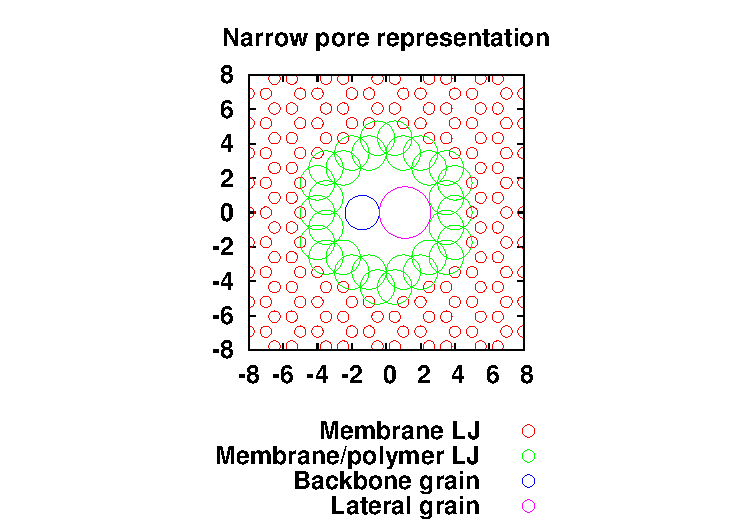
\includegraphics[width=0.9\textwidth]{thinpore.pdf}


\caption[Polymère structuré et pore étroit]{Pore étroit utilisé pour la translocation de notre polymère structuré. Les tailles des différents grains sont respectées. }
\label{porethin}

\end{center}
\end{figure}

\begin{figure}[H]
\begin{center}
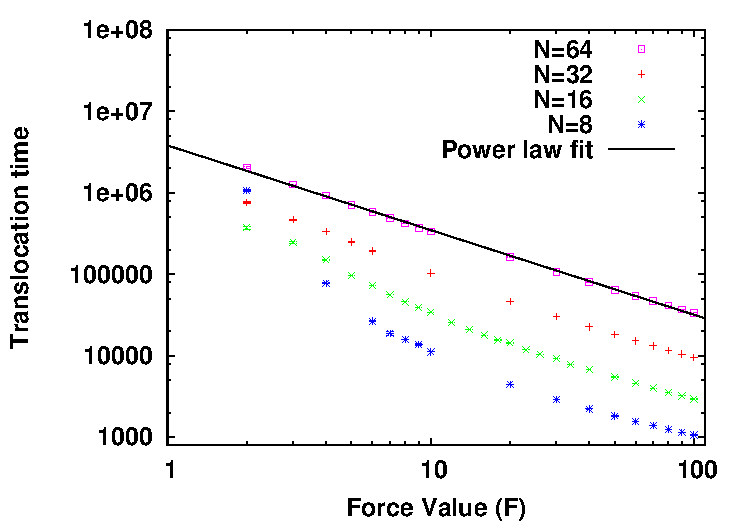
\includegraphics[width=0.9\textwidth]{sptransloc.pdf}
\caption[Temps de translocation du polymère structuré avec un pore étroit]{sf.}
\label{sptransloc}
\end{center}
\end{figure}

\begin{figure}[H]
\begin{center}
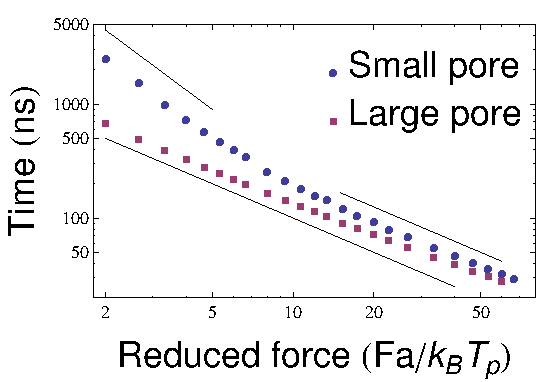
\includegraphics[width=0.9\textwidth]{poresizecomp.pdf} 
\caption[Temps de translocation du polymère structuré, comparaison]{Comparaison}
\label{compporesize}
\end{center}
\end{figure}



\begin{figure}[H]
\begin{center}
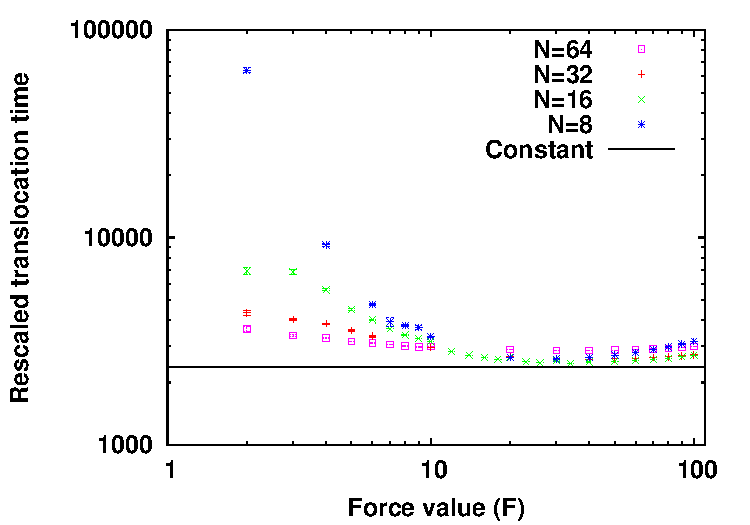
\includegraphics[width=0.9\textwidth]{sptransloctaufresc.pdf}
\caption[Temps de translocation réajusté du polymère structuré et pore étroit]{sf.}
\label{sptransloctaufresc}
\end{center}
\end{figure}

\begin{figure}[H]
\begin{center}
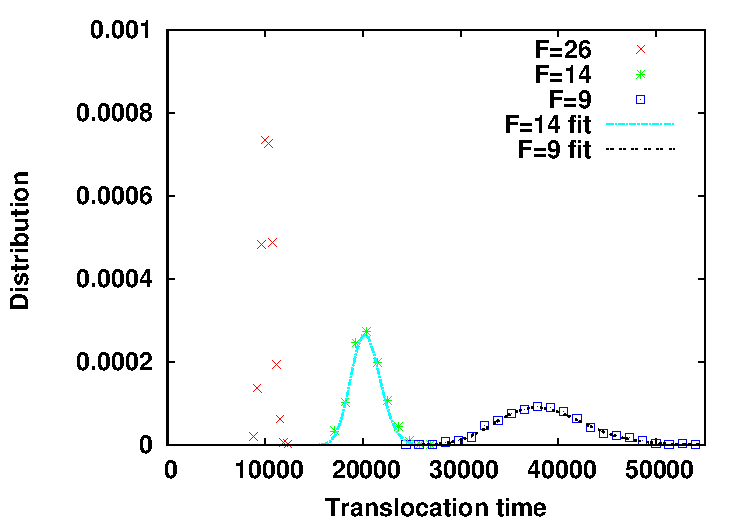
\includegraphics[width=0.9\textwidth]{distribsmallpore.pdf} 
\caption[Distribution des temps de translocation du polymère structuré avec un pore étroit]{distrib}
\label{smallporedistrib}
\end{center}
\end{figure}




\begin{figure}[H]
\begin{center}
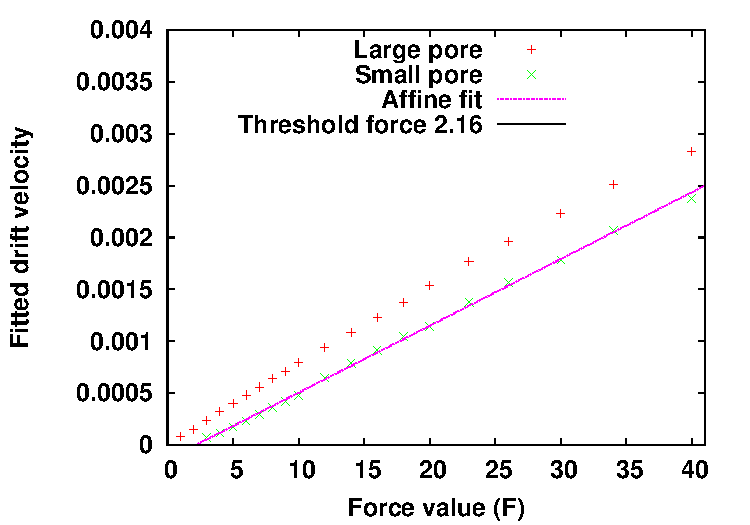
\includegraphics[width=0.9\textwidth]{structuredporesfirction.pdf} 
\caption[Différence de friction entre les pores]{Comparaison friction}
\label{compporesizefriction}
\end{center}
\end{figure}




Nous étudions dorénavant l'effet d'une membrane fixe munie d'un nanopore étroit qui va induire un frottement plus important. Le nanopore est créé en supprimant uniquement 24 grains au centre cette fois ci. Le pore a été choisi suffisamment étroit pour empêcher les monomères de passer de front, ils devront se déformer pour permettre le passage du grain latéral, plus volumineux.\\

Encore une fois, nous observons les deux régimes précédents. Cependant la frontière semble apparaitre plus tard à cause du frottement, ce qui diminue la force effective appliquée sur le polymère ($F_{eff}=F-\epsilon _{pore})$. Les mêmes lois d'échelles sont observées à forte force ( $\tau \propto 1/F$ puis $\tau \propto F^{(1/\nu) -2}$).\\

 Une grande différence s'observe dans le cas de l'application de forces faibles. Comme la Figure \ref{thinpore} le suggère, les translocations n'ont pas pu être menées à bien pour des forces inférieures à l'unité.

Les contraintes stériques choisies entrainent une modification de la barrière d'énergie. La translocation des grains par groupe de trois (1 grain latéral volumineux à la fois), comme nous l'illustrerons dans la section suivante (Figure \ref{temperature}), corrobore une hypothèse de déformation de la barrière entropique en dents de scies décroissante. Cette modification est significative puisqu'elle empêche complétement la translocation si la force appliquée est trop faible, elle semble aussi être responsable du comportement inattendu décrit dans la Figure \ref{thinpore}.

Le cas $N=8$ présente encore une fois des problèmes. Lorsque la force est trop faible, les polymères ne pénètrent pas à travers la membrane. Dans le cas de $N=8$, la force est à peine suffisante pour permettre la translocation et n'est pas prépondérente par rapport au bruit thermique. Le polymère passe alors un temps important à rebondir sur le pore avant d'entamer la translocation. Le temps de translocation est alors fortement surévalué (un point a été conservé sur la Figure \ref{thinpore}, pour illustrer ce problème).





Nous allons maintenant nous intéresser à l'influence des propriétés vibrationnelles du graphène sur la translocation.



